% !TEX root = ../../Dissertation.tex

\begin{refsection}

\chapter[Titanium Digermanium \ch{T\lowercase{i}G\lowercase{e}2}]{Electronic Structures of Titanium Digermanium and Its Anion} \label{TiGe2}


\definecolor{shadecolor}{gray}{0.85}
\begin{shaded}
\textbf{This chapter is based on the paper:}\\
Pham, L. N.; Nguyen, M. T. Titanium Digermanium: Theoretical Assignment of Electronic Transitions Underlying Its Anion Photoelectron Spectrum. \textit{J. Phys. Chem. A} \textbf{2017}, 121, 1940–1949.  \textit{Reprinted with permission from Journal of Chemical Theory and Computation. Copyright 2018. American Chemical Society.} \textcolor{blue}{The \href{https://pubs.acs.org/doi/suppl/10.1021/acs.jpca.7b00245/suppl_file/jp7b00245_si_001.pdf}{Supporting Information} is available online}.

\emph{My contribution to this work was theoretical calculations, data analysis, discussion, writing of the first draft and revision.}
\newpage
\end{shaded}




\section{Introduction}



Germanium is well-known for its use as semiconductor materials in electronic devices. \cite{c4:1, c4:2, c4:3} Because of the high p-type mobility, germanium has been placed under consideration for potential future high-performance electronic transistors. \cite{c4:1} Similar to silicon-based materials, metal-doped germanium materials are believed to bring in improved properties in comparison to the pure ones. \cite{c4:4, c4:5, c4:6, c4:7, c4:8, c4:9, c4:10, c4:11} In the intensive search for such new materials, several transition metal-doped germanium clusters have been experimentally synthesized and characterized. \cite{c4:12, c4:13, c4:14, c4:15, c4:16, c4:17, c4:18, c4:19, c4:20, c4:21} 




In the above-mentioned experimental syntheses, photoelectron (\acrshort{pe}) spectroscopy has frequently been used as a powerful technique to characterize both geometrical and electronic structures of the clusters found, in conjunction with ab initio quantum chemical calculations. \cite{c4:13, c4:14, c4:15, c4:16, c4:19, c4:21} Accordingly, the existence of several small germanium clusters containing metals has been confirmed. In fact, properties of a few series of metal-doped germanium clusters were systematically reported, \cite{c4:15, c4:16, c4:19, c4:21, c4:22, c4:23} such as \ch{TiGe_n^{-/0}}, \ch{VGe_n^{-/0}}, \ch{CoGe_n^{-/0}}, \ch{RuGe_n^{-/0}}, and \ch{AuGe_n^{-/0}}. Besides, complicated germanium clusters doped with transition or lanthanide metals were also studied. \cite{c4:14} Alongside the lowest ionization energies (\acrshort{ie}s) that are usually responsible for electronic transitions between anionic and neutral ground states recorded in anion \acrshort{pe} spectra, other higher \acrshort{ie}s are obtained as well. These higher \acrshort{ie}s correspond to different excited states of neutral clusters. 




Of the series of germanium clusters doped with transition metals mentioned above, the triatomic anion \ch{TiGe2-} was the simplest cluster to experimentally synthesize and characterize. \cite{c4:22} After being generated in a laser vaporization source, the
mass-selected anion \ch{TiGe2-} was guided into the laser beam with an energy of 266 nm to measure detachment energies. Measurement at this level of photon energy showed four ionization bands in the \acrshort{pe} spectrum of \ch{TiGe2-}. The lowest band had an adiabatic detachment energy (\acrshort{ade}) of 0.78 eV and a vertical detachment energy (\acrshort{vde}) of 1.06 eV. There were also three more bands observed with higher electron binding energies of 1.44, 2.05, and 2.49 eV. Previous \acrshort{dft} calculations using both B3LYP and HSE06 functionals on geometrical structures of \ch{TiGe2^{-/0}} pointed out that both states have a cyclic C$_{2v}$ structure. \cite{c4:22, c4:24} The anionic and neutral ground electronic states were believed to be the $^2$A$_2$ and $^3$B$_1$, respectively. \cite{c4:22} Therefore, the lowest-lying band in the \acrshort{pe} spectrum of \ch{TiGe2-} was assigned to the $^2$A$_2$ $\longrightarrow$ $^3$B$_1$ transition. 




As far as we are aware, there is no information about the excited states and corresponding electronic transitions underlying the bands in \acrshort{pe} spectra of any germanium cluster containing transition metals. As \ch{TiGe2-} is the simplest experimentally obtained species among the metal-doped germanium clusters reported, we surprisingly recognized from preliminary calculations that a low-spin doublet state cannot be the ground state of the anion \ch{TiGe2-}, as reported in the previous \acrshort{dft} study. In this context, we set out to more deeply investigate the electronic structure of the triatomic \ch{TiGe2} in both anionic and neutral states. All electronic states of the neutral \ch{TiGe2} were determined in order to elucidate the four bands seen in the \acrshort{pe} spectrum of \ch{TiGe2-}. 




\section{Computational Details}


As \ch{TiGe2^{-/0}} clusters have two low-lying isomers, being the cyclic and the linear ones, depicted in Figure \ref{fig4:tige2}, the simplest step of our calculation scheme is to confirm the higher stability of the cyclic isomer in both anionic and neutral forms. \cite{c4:22, c4:24} Because our preliminary calculations showed that the M06-L functional appears to be more suitable than other popular functionals in the determination of \acrshort{ie}s for \ch{TiGe2-} and this functional also performs well for transition metals, \cite{c4:25, c4:26} we use the M06-L functional\cite{c4:26} to rapidly locate the equilibrium geometries of two low-lying isomers (Figure \ref{fig4:tige2}) of \ch{TiGe2^{-/0}}. Because the primary purpose of this step is to identify the global energy minimum, geometries of all spin multiplicities from singlet to octet of \ch{TiGe2^{-/0}} are taken into account during \acrshort{dft} geometry optimizations. All unrestricted open-shell \acrshort{dft} calculations in this step are carried out using the Gaussian 09E.01 suite of program packages \cite{c4:27} and employ the correlation consistent polarized triple-$\zeta$ basis set aug-cc-pVTZ,\cite{c4:28, c4:29} unless otherwise noted. Although the cyclic isomers of \ch{TiGe2^{-/0}} previously proved to have spatial symmetry of C$_{2v}$, \cite{c4:22} no geometrical symmetry is imposed during this optimization step, which allows both linear and cyclic low-lying isomers to be fully optimized (Figure \ref{fig4:tige2}). 



\begin{figure}[htb!]
	\centering
	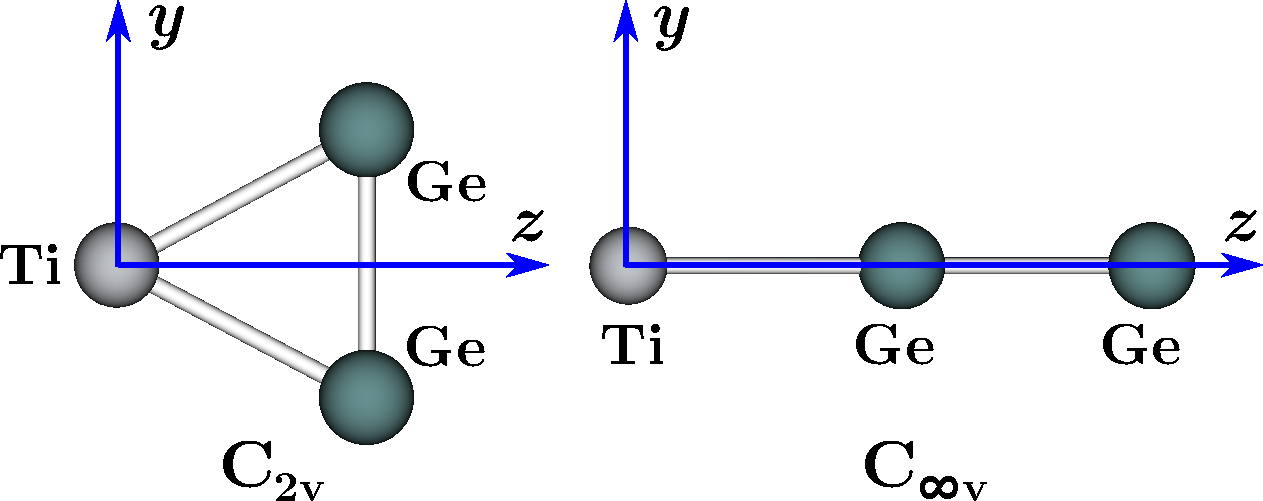
\includegraphics[width=0.5\textwidth]{tige2}
	\caption{Two low-lying isomers of \ch{TiGe2^{-/0}} and the Cartesian coordinate axes.}
	\label{fig4:tige2}
\end{figure} 



As our investigated systems contain transition metals, all spatial states of \ch{TiGe2^{-/0}} are again optimized at a higher level of theory, namely, the \acrshort{caspt2}, \cite{c4:30} which is able to better treat correlation energy. To perform such calculations, predefined coordinate systems should be applied to the target \ch{TiGe2^{-/0}}. As seen in Figure \ref{fig4:tige2}, for the cyclic isomer, the molecular plane is chosen to be the yz-plane, and the titanium atom is located at the origin of the Cartesian coordinate system; the \ch{Ge-Ge} bonding is perpendicular to the z-axis. The active space and numbers of electrons included in the active space should also be defined. For germanium, all of the 4p valence orbitals are treated in the active space because our probing calculations indicated that 4s and inner orbitals do not involve in electronic transitions. As for titanium, six valence orbitals including one 4s and five 3d ones are taken into account. In total, 12 orbitals in the active space are statically correlated. Because titanium has a total of four electrons in the 4s and 3d subshells and there are two electrons in the 4p subshell of germanium, the total number of electrons in the active space amounts to eight for the neutral \ch{TiGe2} and nine for the anion \ch{TiGe2-}. The \acrshort{ano}-RCC basis set with [7s6p4d3f2g] contraction for titanium \cite{c4:31} and [6s5p3d1f] contraction for germanium \cite{c4:32} is used for this geometry optimization step with the assistance of the Molcas 8.1 package. \cite{33}






To increase the reliability of relative energies in the determination of the global ground states, one more geometry optimization using the single-reference functional M06-L is then conducted in conjunction with the triple-$\zeta$ basis set aug-cc-pVTZ-DK on the basis of leading configurations drawn above. In addition, single-point calculations using \acrshort{caspt2}-optimized geometries are also carried out, utilizing the coupled-cluster theory \acrshort{rccsd}(T) and the n-electron valence state perturbation theory \acrshort{nevpt2}. The latter is used to synergistically draw out the ground states of \ch{TiGe2^{-/0}} because a few lower spin states cannot be described with single-reference methods, and more importantly, there is a competition for the anionic ground state at the \acrshort{caspt2} level among the energetically nearly degenerate states. For the sake of convenience, \acrshort{rccsd}(T) calculations use the same triple-$\zeta$ basis set used in M06-L optimizations. Multireference single-point \acrshort{casscf}/\acrshort{nevpt2} \cite{c4:34} calculations employ the larger quintuple-$\zeta$ basis set, aug-cc-pV5Z-DK. All obtained energies for low-lying states allow us to confidently identify the ground states of both anionic and neutral forms. Once the ground states are identified, both \acrshort{ade}s and \acrshort{vde}s can be evaluated. The difference between \acrshort{vde} and \acrshort{ade} procedures concerns the geometries of final states, which are the \acrshort{caspt2}-optimized geometrical parameters of every involved neutral state and the \acrshort{caspt2} optimal geometry of the anionic initial state for \acrshort{ade}s and \acrshort{vde}s, respectively. To efficiently reproduce the correlation energy at single-reference levels, such as M06-L and \acrshort{rccsd}(T), we increase the basis set size to the quintuple-$\zeta$ aug-cc-pV5Z-DK when evaluation of \acrshort{ade}s and \acrshort{vde}s is conducted. All single-reference \acrshort{dft} and \acrshort{rccsd}(T), and \acrshort{casscf}/\acrshort{nevpt2} calculations are carried out using Molpro 2012. \cite{c4:35} Because both germanium and titanium are heavy elements, all electron scalar relativistic effects are taken into account by making use of the second-order Douglas-Kroll-Hess Hamiltonian (denoted as DK). \cite{c4:36} All relative energies are derived without \acrshort{zpe} corrections because for these small species their \acrshort{zpe}s are quite similar and do not significantly affect the relative positions on the potential surfaces. \cite{c4:37}





It should be mentioned that the true energy minima obtained from geometrical optimizations at the M06-L and \acrshort{caspt2} levels are confirmed by subsequent vibrational frequency analyses (without any negative vibrational frequency). This step not only ensures the identity of each structure, but also provides us with coordinates of the vibration normal modes, which are in turn used for multidimensional Franck-Condon factor integrations. Our basic evaluation shows that single-reference methods are not energetically efficient to describe \ch{TiGe2^{-/0}}, and hence, we use vibrational frequencies of the normal modes computed at the \acrshort{caspt2} level. At this level, several final states that are responsible for the bands in the \acrshort{pe} spectrum of \ch{TiGe2-} can be accessed, and their normal modes of vibrations are numerically obtained. The multidimensional Franck-Condon factors are simulated with the MolFC code. \cite{c4:38}





\section{Results and Discussion}



\subsection{Ground and Low-Lying States of \ch{TiGe2^{-/0}}.}




Relative energies of the cyclic and linear isomers in several spin multiplicities are collected and graphically visualized in Figure \href{https://pubs.acs.org/doi/suppl/10.1021/acs.jpca.7b00245/suppl_file/jp7b00245_si_001.pdf}{\textcolor{blue}{S1}} of the \href{https://pubs.acs.org/doi/suppl/10.1021/acs.jpca.7b00245/suppl_file/jp7b00245_si_001.pdf}{\textcolor{blue}{Supporting Information}} (available online). The cyclic isomer is confirmed to be more stable than the linear counterpart for both anionic and neutral forms. For the anion, a quartet state of the cyclic isomer emerges as the most stable one using the M06-L functional. Surprisingly, this result completely disagrees with the conclusion previously reported \cite{c4:22} that the doublet state $^2$A$_2$ of the cyclic isomer is the most stable anionic form. Such a discrepancy in the identity of the anionic ground state stimulates us to proceed a further step to construct more elaborated \ch{TiGe2} hypersurfaces in both low- and high-spin states. 



Figure \href{https://pubs.acs.org/doi/suppl/10.1021/acs.jpca.7b00245/suppl_file/jp7b00245_si_001.pdf}{\textcolor{blue}{S2a}} (\href{https://pubs.acs.org/doi/suppl/10.1021/acs.jpca.7b00245/suppl_file/jp7b00245_si_001.pdf}{\textcolor{blue}{ESI}}) shows the adiabatic potential surface of both doublet and quartet states using the M06-L functional when the 
\ch{Ti-Ge} bond length increases from 2.1 to 3.1 \AA. Both potential energy surfaces strongly support the conclusion mentioned above. Therefore, a quartet state can be probed as the anionic ground state. In addition, one can rule out the high-spin states such as the sextet and octet because they are located at quite high energy levels on the potential surface of \ch{TiGe2-}. Thus, these spin states are ignored in the following discussion. 



Turning now to the neutral form, a triplet cycle is clearly the most stable isomer. Conversely, the high-spin septet states are characterized to be quite high relative energies in comparison to the triplet state. This high-spin state as well as the linear isomer is therefore not considered in subsequent steps because they are not significantly populated in photodetachment processes. 




In order to safely identify the global ground states, further optimization is performed using two methods, \acrshort{caspt2} and M06-L, and single-point electronic energies of the obtained states at the \acrshort{rccsd}(T) and \acrshort{casscf}/\acrshort{nevpt2} levels are also calculated. These relative energies and \acrshort{caspt2} geometries are tabulated in Table \ref{tbl4:RE}. In this step, all methods consistently identify the $^4$B$_1$ and $^3$B$_1$ states as the ground states of the anion and the neutral, respectively. Both single-reference methods also point toward the $^4$B$_1$ as the energetically lowest anionic state. M06-L and \acrshort{rccsd}(T) estimate that the $^4$B$_1$ is 0.33 and 0.12 eV more  stable than the first excited state $^2$A$_1$ of the anion. There is also a significant difference of 0.19 eV between the $^4$B$_1$ and the second excited state $^2$A$_2$ of \ch{TiGe2-} at the \acrshort{rccsd}(T) level. Note that the $^2$A$_2$ was assigned to be the ground anionic state in a previous study.\cite{c4:22}




\begin{table}[htb!]
	\centering
	%\small   
	\begin{threeparttable} 
	\caption{Determination of Ground States of Both Anionic and Neutral \ch{TiGe2} at Different Levels}
	\label{tbl4:RE}
	\begin{tabular}{@{}lcl>{\centering\arraybackslash}p{0.9cm}cl>{\centering\arraybackslash}p{0.7cm}>{\centering\arraybackslash}p{1.1cm}>{\centering\arraybackslash}p{1cm}c@{}}
		\toprule
		\multirow{2}{*}{species} & \multirow{2}{*}{state} &  & \multicolumn{2}{c}{\acrshort{caspt2} geometry (\AA)} &  & \multicolumn{4}{c}{relative energy (eV)\tnote{(a)}} \\ \cmidrule(lr){4-5} \cmidrule(l){7-10}  
		&   &  & Ti-Ge  & Ge-Ge  &  & M06L   & \acrshort{rccsd}(T)   & \acrshort{nevpt2}   & \acrshort{caspt2}   \\ \cmidrule(r){1-2} \cmidrule(lr){4-5} \cmidrule(l){7-10} 
\begin{tabular}[c]{@{}l@{}}cyclic \\ \ch{TiGe2-}\end{tabular}  & $^2$A$_1$    &  & 2.44   & 2.50    &  & 0.33    & 0.12       & 0.02     & 0.01     \\
		& $^2$B$_1$         &  & 2.50      & 2.35   &  &         &        & 0.22     & 0.25     \\
		& $^2$B$_2$         &  & 2.47      & 2.36   &  & 0.70    & 0.31   & 0.26     & 0.28     \\
		& $^2$A$_2$         &  & 2.40      & 2.58   &  & 0.33    & 0.19   & 0.06     & 0.08     \\
		& $^4$A$_1$         &  & 2.46      & 2.42   &  & 0.43    & 0.47   & 0.39     & 0.39     \\
		& $^4$B$_1$         &  & 2.50      & 2.35   &  & 0.00    & 0.00   & 0.00     & 0.00     \\
		& $^4$B$_2$         &  & 2.49      & 2.37   &  & 0.48    & 0.18   & 0.22     & 0.26     \\
		& $^4$A$_2$         &  & 2.57      & 2.33   &  & 0.42    & 0.34   & 0.49     & 0.38     \\ 
\begin{tabular}[c]{@{}l@{}}cyclic \\ \ch{TiGe2}\end{tabular}   & $^1$A$_1$    &  & 2.41 & 2.48               &  & 1.81    & 1.65       & 1.50     & 1.38     \\
		& $^1$B$_1$         &  & 2.42      & 2.43   &  &         &        & 1.57     & 1.35     \\
		& $^1$B$_2$         &  & 2.45      & 2.39   &  &         &        & 1.62     & 1.33     \\
		& $^1$A$_2$         &  & 2.44      & 2.54   &  &         &        & 2.31     & 2.15     \\
		& $^3$A$_1$         &  & 2.59      & 2.33   &  & 2.16    & 2.74   & 2.18     & 2.07     \\
		& $^3$B$_1$         &  & 2.43      & 2.41   &  & 1.15    & 1.33   & 1.07     & 0.90     \\
		& $^3$B$_2$         &  & 2.44      & 2.39   &  & 1.37    & 1.37   & 1.14     & 0.94     \\
		& $^3$A$_2$         &  & 2.54      & 2.34   &  & 1.94    & 1.98   & 2.10     & 1.98     \\
		& $^5$A$_1$         &  & 2.57      & 2.33   &  & 2.19    & 2.76   & 2.53     & 2.37     \\
		& $^5$B$_1$         &  & 2.54      & 2.54   &  & 2.54    & 2.72   & 2.53     & 2.28     \\
		& $^5$B$_2$         &  & 2.79      & 2.25   &  & 2.64    & 2.65   & 2.92     & 2.75     \\
		& $^5$A$_2$         &  & 2.81      & 2.34   &  & 2.82    & 2.88   & 3.34     & 3.01     \\ \bottomrule
	\end{tabular}
	\begin{tablenotes}
		\item[(a)] \acrshort{rccsd}(T) and \acrshort{nevpt2} energies were obtained with the use of \acrshort{caspt2}-optimized geometries. All relative energies were determined without \acrshort{zpe} corrections.
	\end{tablenotes}
	\end{threeparttable}
\end{table}



The situation gets more complex at the \acrshort{caspt2} and \acrshort{nevpt2} levels, in which the ground, first, and second excited states of \ch{TiGe2-} are determined to lie very close to each other. The $^2$A$_1$ state is only 0.01 and 0.02 eV higher than the $^4$B$_1$ at the \acrshort{caspt2} and \acrshort{nevpt2} levels, respectively. For the $^2$A$_2$ state, the \acrshort{caspt2} and \acrshort{nevpt2} produce relative energies of 0.08 and 0.06 eV, respectively. Accordingly, these three states are quasi-degenerate at multireference theory.	




Such a degeneracy of many states is encountered as well in the neutral \ch{TiGe2}. Our calculated relative energies confirm the neutral ground state $^3$B$_1$, in full agreement with previous conclusions, \cite{c4:22, c4:24} even though both $^3$B$_1$ and $^3$B$_2$ states seem to be nearly degenerate at several levels (\acrshort{rccsd}(T), \acrshort{caspt2}, and \acrshort{nevpt2}). The $^3$B$_1$ state is $\sim$0.05 eV lower in energy than the $^3$B$_2$. With regard to higher-lying excited states, three singlet states $^1$A$_1$, $^1$B$_1$, and $^1$B$_2$ are determined to lie higher than the ground $^3$B$_1$ by an amount of $\sim$0.50 eV at both \acrshort{caspt2} and \acrshort{nevpt2} levels. Interestingly, these three singlet states seem also nearly degenerate, and hence, this could result in a complicated determination of electronic transitions (final states).



\subsection{Electronic Structures and One-Electron Electronic Transitions}



Investigation into the electronic structure of both anionic and neutral ground states allows us to know whether the one-electron transition between two ground states, which gives rise to the lowest recorded band in the anion spectrum of \ch{TiGe2-}, is possible. The leading configurations of many states obtained from \acrshort{casscf} wave functions and their weights are given in Table \ref{tbl4:ldconfig}.


Let us first thoroughly examine the anionic ground state because most bands that appeared in the \acrshort{pe} spectrum originate from it. The anionic state $^4$B$_1$ is determined by three singly occupied orbitals a$_1$, b$_2$, and a$_2$ and three doubly occupied ones as noted in Table \ref{tbl4:ldconfig}. The three singly occupied orbitals are largely contributed to by valence orbitals of titanium. On the basis of the \acrshort{casscf} wave function, the totally symmetric orbital 19a$_1$, one of three singly occupied molecular orbitals (\acrshort{mo}s), is composed mainly of the metallic 4s orbital, while the other two \acrshort{mo}s 14b$_2$ and 5a$_2$ are dominantly contributed to by 3d$_{yz}$ and 3d$_{xy}$ orbitals, respectively. The doubly occupied \acrshort{mo}s 17a$_1$, 18a$_1$, and 7b$_1$ are based on the six 4p orbitals of the \ch{Ge2} moiety. Similar to the electronic structure of \ch{Ge2}, \cite{c4:39} the six 4p orbitals of the \ch{Ge2} moiety can form one bonding $\sigma_g$ and two $\pi_u$ \acrshort{mo}s. With graphic assistance from the orbital shape in Figure \ref{fig4:orbs}, it is able to exactly map the original components of these \acrshort{mo}s. Apparently, the two $\pi_u$ orbitals 18a$_1$ and 7b$_1$ are built up from 4p$_z$ and 4p$_x$ atomic orbitals (\acrshort{ao}s) of Ge, and the $\sigma_g$, being the 17a$_1$, is from an overlap between two 4p$_y$ \acrshort{ao}s. For the sake of convenience in solving \acrshort{pe} bands in a following step, the leading configuration of $^4$B$_1$ can be formulated in another form as [\ldots $\sigma_g^2$ $\pi_{4p_z}^2$ 4$s^1$ $\pi_{4p_x}^2$ 3$d_{yz}^1$ 3$d_{xy}^1$].



\begin{figure}[htb!]
	\centering
	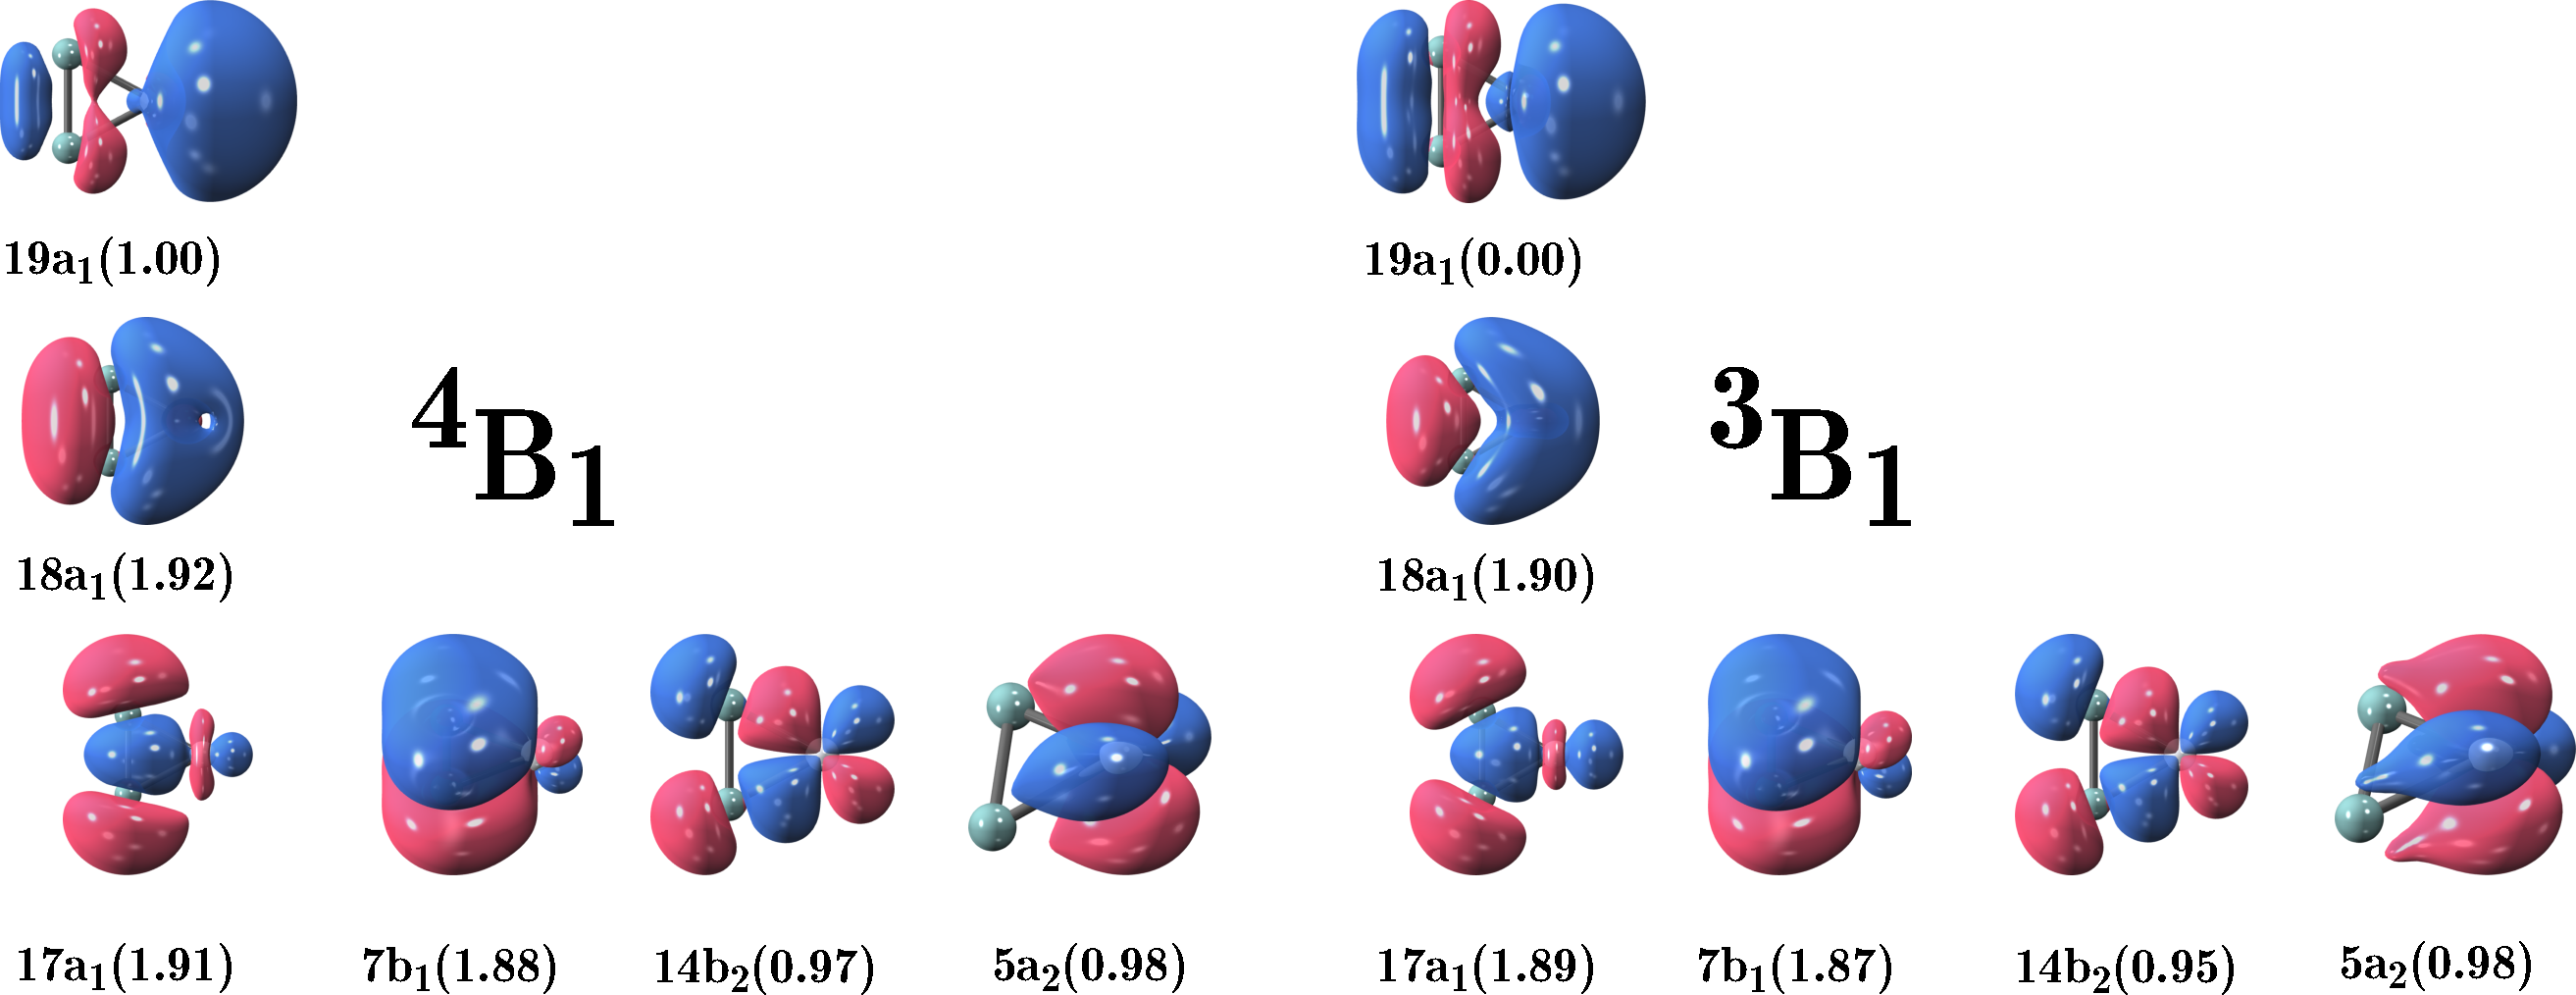
\includegraphics[width=\textwidth]{4B1-3B1-orbitals}
	\caption{Occupied pseudonatural orbitals in the active spaces of states $^4$B$_1$ and $^3$B$_1$ (\acrshort{casscf} wave functions). The average occupation numbers are given in parentheses. The metal atom Ti is located on the right-hand side.} 
	\label{fig4:orbs}
\end{figure} 



\begin{center}
\begin{landscape} 
	\begin{longtable}{@{}ccccc@{}} 
	%\footnotesize 
	\caption{Leading Configurations of the Two Most Stable Anionic Ground States and of Neutral Ones}	\\
	\toprule
	state  & leading configuration     & weight (\%)  	  & transition     & ionization orbital     \\ \midrule 
	\endfirsthead
	\multicolumn{5}{c}%
	{{\tablename\ \thetable{} -- continued from previous page}} \\
	\toprule
	state  & leading configuration     & weight (\%)  	  & transition      & ionization orbital     \\ \midrule 
	\endhead
	\bottomrule \multicolumn{5}{r}{{Continued on next page}} \\   
	\endfoot	
	\bottomrule 
	\endlastfoot 
	$^4$B$_1$    & 17a$_1^2$ 18a$_1^2$ 19a$_1^1$ 20a$_1^0$ 21a$_1^0$ 7b$_1^2$ 8b$_1^0$ 14b$_2^1$ 5a$_2^1$  & 83   &    &                    \\
	$^2$A$_1$    & 17a$_1^2$ 18a$_1^2$ 19a$_1^0$ 20a$_1^1$ 21a$_1^0$ 7b$_1^2$ 8b$_1^0$ 14b$_2^2$ 5a$_2^0$  & 71   &    &                    \\
	$^2$A$_2$    & 17a$_1^2$ 18a$_1^2$ 19a$_1^0$ 20a$_1^0$ 21a$_1^0$ 7b$_1^2$ 8b$_1^0$ 14b$_2^2$ 5a$_2^1$  & 73   &    &                    \\
	\multirow{2}{*}{$^1$A$_1$} & \multirow{2}{*}{17a$_1^2$ 18a$_1^2$ 19a$_1^0$ 20a$_1^0$ 21a$_1^0$ 7b$_1^2$ 8b$_1^0$ 14b$_2^2$ 5a$_2^0$} & \multirow{2}{*}{76} & $^2$A$_1$ $\longrightarrow$ $^1$A$_1$  & 20a$_1$ (Ti: 3d$_{x^2-y^2}$) \\
						 &    &  & $^2$A$_2$ $\longrightarrow$ $^1$A$_1$  & $^5$a$_2$    (Ti: 3d$_{xy}$)  \\
	$^1$B$_1$    & 17a$_1^2$ 18a$_1^2$ 19a$_1^0$ 20a$_1^0$ 21a$_1^0$ 7b$_1^2$ 8b$_1^0$ 14b$_2^1$ 5a$_2^1$  & 74   &    &                    \\
	$^1$B$_2$    & 17a$_1^2$ 18a$_1^2$ 19a$_1^0$ 20a$_1^1$ 21a$_1^0$ 7b$_1^2$ 8b$_1^0$ 14b$_2^1$ 5a$_2^0$  & 72   &    &                    \\
	$^1$A$_2$    & 17a$_1^2$ 18a$_1^1$ 19a$_1^0$ 20a$_1^0$ 21a$_1^0$ 7b$_1^2$ 8b$_1^0$ 14b$_2^2$ 5a$_2^1$  & 57   &    &                    \\
	$^3$A$_1$    & 17a$_1^2$ 18a$_1^2$ 19a$_1^0$ 20a$_1^1$ 21a$_1^1$ 7b$_1^2$ 8b$_1^0$ 14b$_2^0$ 5a$_2^0$  & 85   &    &                    \\
	\multirow{2}{*}{$^3$B$_1$} & \multirow{2}{*}{17a$_1^2$ 18a$_1^2$ 19a$_1^0$ 20a$_1^0$ 21a$_1^0$ 7b$_1^2$ 8b$_1^0$ 14b$_2^1$ 5a$_2^1$} & \multirow{2}{*}{80} & $^4$B$_1$ $\longrightarrow$ $^3$B$_1$  & 19a$_1$ (Ti: 4s)      \\
						 &    &  & $^2$A$_2$ $\longrightarrow$ $^3$B$_1$  & 14b$_2$ (Ti: 3d$_{yz}$)    \\
	1$^3$B$_2$   & 17a$_1^2$ 18a$_1^2$ 19a$_1^0$ 20a$_1^1$ 21a$_1^0$ 7b$_1^2$ 8b$_1^0$ 14b$_2^1$ 5a$_2^0$  & 83   &    &                    \\
	2$^3$B$_2$   & 17a$_1^2$ 18a$_1^2$ 19a$_1^1$ 20a$_1^0$ 21a$_1^0$ 7b$_1^2$ 8b$_1^0$ 14b$_2^1$ 5a$_2^0$  & 41   & $^4$B$_1$ $\longrightarrow$ 2$^3$B$_2$ & 5a$_2$ (Ti: 3d$_{xy}$)   \\
	3$^3$B$_2$   & 17a$_1^2$ 18a$_1^2$ 19a$_1^0$ 20a$_1^0$ 21a$_1^0$ 7b$_1^2$ 8b$_1^1$ 14b$_2^0$ 5a$_2^1$  & 44   &    &                    \\
	1$^3$A$_2$   & 17a$_1^2$ 18a$_1^2$ 19a$_1^0$ 20a$_1^0$ 21a$_1^1$ 7b$_1^2$ 8b$_1^0$ 14b$_2^0$ 5a$_2^1$  & 86   &    &                    \\
	2$^3$A$_2$   & 17a$_1^2$ 18a$_1^2$ 19a$_1^1$ 20a$_1^0$ 21a$_1^0$ 7b$_1^2$ 8b$_1^0$ 14b$_2^0$ 5a$_2^1$  & 60   & $^4$B$_1$ $\longrightarrow$ 2$^3$A$_2$ & 14b$_2$ (Ti: 3d$_{yz}$)    \\
	3$^3$A$_2$   & 17a$_1^2$ 18a$_1^2$ 19a$_1^0$ 20a$_1^0$ 21a$_1^0$ 7b$_1^2$ 8b$_1^1$ 14b$_2^1$ 5a$_2^0$  & 79   &    &                    \\
	1$^5$A$_1$   & 17a$_1^2$ 18a$_1^2$ 19a$_1^0$ 20a$_1^0$ 21a$_1^0$ 7b$_1^2$ 8b$_1^1$ 14b$_2^1$ 5a$_2^1$  & 83   &    &                    \\
	2$^5$A$_1$   & 17a$_1^2$ 18a$_1^2$ 19a$_1^1$ 20a$_1^0$ 21a$_1^0$ 7b$_1^1$ 8b$_1^0$ 14b$_2^1$ 5a$_2^1$  & 78   & $^4$B$_1$ $\longrightarrow$ 2$^5$A$_1$ & 7b$_1$ (Ge: 4p$_x$)      \\
	3$^5$A$_1$   & 17a$_1^2$ 18a$_1^2$ 19a$_1^0$ 20a$_1^0$ 21a$_1^1$ 7b$_1^1$ 8b$_1^0$ 14b$_2^1$ 5a$_2^1$  & 76   &    &                    \\
	1$^5$B$_1$   & 17a$_1^2$ 18a$_1^2$ 19a$_1^0$ 20a$_1^0$ 21a$_1^0$ 7b$_1^1$ 8b$_1^1$ 14b$_2^1$ 5a$_2^1$  & 81   &    &                    \\
	2$^5$B$_1$   & 17a$_1^2$ 18a$_1^1$ 19a$_1^1$ 20a$_1^0$ 21a$_1^0$ 7b$_1^2$ 8b$_1^0$ 14b$_2^1$ 5a$_2^1$  & 74   & $^4$B$_1$ $\longrightarrow$ 2$^5$B$_1$ & 18a$_1$ (Ge: 4p$_y$)     \\
	3$^5$B$_1$   & 17a$_1^1$ 18a$_1^2$ 19a$_1^1$ 20a$_1^0$ 21a$_1^0$ 7b$_1^2$ 8b$_1^0$ 14b$_2^1$ 5a$_2^1$  & 75   & $^4$B$_1$ $\longrightarrow$ 3$^5$B$_1$ & 17a$_1$ (Ge: 4p$_z$)     \\
	1$^5$B$_2$   & 17a$_1^2$ 18a$_1^1$ 19a$_1^1$ 20a$_1^1$ 21a$_1^0$ 7b$_1^2$ 8b$_1^0$ 14b$_2^1$ 5a$_2^0$  & 89   &    &                    \\
	1$^5$A$_2$   & 17a$_1^2$ 18a$_1^2$ 19a$_1^1$ 20a$_1^1$ 21a$_1^0$ 7b$_1^1$ 8b$_1^0$ 14b$_2^1$ 5a$_2^0$  & 91   &    &                     
	\label{tbl4:ldconfig}
\end{longtable}                                                                          
\end{landscape}
\end{center}


As analyzed above, the anionic $^2$A$_1$ is a nearly degenerate state of the state $^4$B$_1$ at both levels \acrshort{caspt2} and \acrshort{nevpt2}. In this situation, multireference methods are expected to reproduce more reliable results because many states of \ch{TiGe2^{-/0}} cannot be well-described by single-reference wave functions. Therefore, we believe that the $^2$A$_1$ state can be somehow populated in experiment and thereby involved in the spectral appearance. As expected, the leading configuration of the $^2$A$_1$ state (Table \ref{tbl4:ldconfig}) is dominated by the singly occupied orbital 20a$_1$. The relevant pseudonatural orbital is constructed from a primary part 3d$_{x^2-y^2}$ and a minor amount of 4s, which are both valence orbitals of titanium. The four doubly occupied orbitals of $^2$A$_1$ include the 17a$_1$, 18a$_1$, 7b$_1$, and 14b$_2$. Thus, electronic components are chiefly the same as those of the anionic ground state $^4$B$_1$. In terms of orbital components, the nearly degenerate state $^2$A$_1$ can be rewritten as [\ldots $\sigma_g^2$ $\pi^2_{4p_z}$ 3$d_{(x^2-y^2)}^1$ $\pi_{4p_x}^2$ 3$d^2_{yz}$].


Normally, the lowest-lying band in an anion \acrshort{pe} spectrum is the result of a one-electron transition between the anionic and neutral ground states. Let us briefly consider the electronic structure of the neutral $^3$B$_1$. In Table \ref{tbl4:ldconfig}, the leading orbital configuration of the $^3$B$_1$ shows a similarity of its orbital components in comparison to the anionic state $^4$B$_1$. Indeed, the neutral state has two singly occupied \acrshort{mo}s 14b$_2$ and 5a$_2$, together with three doubly occupied \acrshort{mo}s 17a$_1$, 18a$_1$, and 7b$_1$ (quite similar to those of $^4$B$_1$). In principle, the electron located in orbital 19a$_1$ of $^4$B$_1$ can be removed, giving rise to the neutral $^3$B$_1$, and therefore, the neutral leading configuration of the state $^3$B$_1$ can be assigned as [\ldots $\sigma_g^2$ $\pi_{4p_z}^2$ 4$s^0$ $\pi_{4p_x}^2$ 3$d_{yz}^1$ 3$d_{xy}^1$]. The 4s electron of titanium can thus be ionized from the anionic state $^4$B$_1$ under the high-energy laser beam to generate neutral $^3$B$_1$.




Within the scope of the treated active spaces, we can predict six possible one-electron ionizations starting from the anionic ground state $^4$B$_1$. Six electrons located in six occupied orbitals can be removed, one by one, to form six corresponding final states, including the neutral ground state $^3$B$_1$. Two 3d \acrshort{mo}s (14b$_2$ and 5a$_2$) can participate in one-electron photodetachment, and the proposed final electronic states are 2$^3$A$_2$ and 2$^3$B$_2$, respectively, whose leading configurations can be found in Table \ref{tbl4:ldconfig}. Out of the metallic valence orbitals, three other one-electron ionizations can individually occur in three doubly occupied orbitals $\sigma_g^2$, $\pi_{4p_z^2}$, and $\pi_{4p_x^2}$, noted as 17a$_1$, 18a$_1$, and 7b$_1$ in the $^4$B$_1$ leading configuration, respectively. The corresponding electronic states are 3$^5$B$_1$, 2$^5$B$_1$, and 2$^5$A$_1$, whose leading configurations are also listed in Table \ref{tbl4:ldconfig}. Apart from the above-mentioned states, other low-lying states cannot theoretically be final states of one-electron photoionization, simply because their electronic structures (as presented by leading configurations) cannot be the final leading configurations of one-electron detachments starting from the anionic ground state. 





The coefficient weights of leading configurations can quantitatively give an additional evaluation of the nature of corresponding states. When a system is well-described with single-reference wave functions, \cite{c4:37} all coefficient weights of leading configurations amount to $\geq$85$\%$ and are nearly equal to each other. For \ch{TiGe2^{-/0}} (Table \ref{tbl4:ldconfig}) most leading configurations of the states potentially taking part in one-electron transitions contribute to the corresponding electronic wave functions with coefficient weights of $\leq$80$\%$. The only one over 80$\%$ (83$\%$ to be accurate) belongs to the anionic ground state $^4$B$_1$. This gives a reason why the anionic ground state, the nearly degenerate state, and all other final low-lying states are not well-described by single-reference wave functions. In other words, single-reference quantum chemical methods are again confirmed to be inappropriate for treating systems like \ch{TiGe2^{-/0}}.





Taking a closer look at electronic structures of the anionic states $^4$B$_1$, $^2$A$_1$, and $^2$A$_2$, remarkable quantitative differences between the leading coefficient weights of $^4$B$_1$ (83$\%$) and those of two other states $^2$A$_1$ and $^2$A$_2$ (71 and 73$\%$, respectively) can be noticed. A difference of >10$\%$ implies that single-reference methods cannot recover the correlation energy of these two excited states well. This explains why the previous single-reference study \cite{c4:22} failed in locating the global ground state of \ch{TiGe2-} on the potential hypersurface. On the basis of \acrshort{caspt2} and \acrshort{nevpt2} relative energies listed in Table \ref{tbl4:RE}, three state $^4$B$_1$, $^2$A$_1$, and $^2$A$_2$ are very close to each other in terms of energy and can accordingly be treated as quasi-degenerate states.






From the analysis above, three states $^4$B$_1$, $^2$A$_1$, and $^2$A$_2$ are energetically close and hence can be populated in the \acrshort{pe} experiment. However, the anions \ch{TiGe2-} were cooled down after being synthesized. On the basis of Maxwell-Boltzmann statistics, the population of $^2$A$_2$ (relative energy of $\sim$0.1 eV at the \acrshort{caspt2} level) is predicted to be negligible, and thus, insignificant intensities of \acrshort{pe} signals originating from this state are expected. Two remaining states have closer relative energies, and the difference is $\sim$0.01 eV. These two states could thus be more populated in the \acrshort{pe} experiment, especially the anionic ground state $^4$B$_1$, and therefore could be taking part in possible electronic transitions underlying bands in the \acrshort{pe} spectrum of \ch{TiGe2-}.






We predict possible final neutral states in the situation that electronic transitions start from the anionic ground state $^4$B$_1$. If the nearly degenerate state $^2$A$_1$ is significantly populated in a \acrshort{pe} experiment, signals of its one-electron ionizations can be observed in the \acrshort{pe} spectrum of \ch{TiGe2-}. The relevant question is thus about the final states. On the basis of all low-lying neutral leading configurations, it is easy to add $^1$A$_1$ to the list of final states. In this case, the unique singly occupied \acrshort{mo} 20a$_1$, also known as 3d$_{x^2-y^2}^1$, of the $^2$A$_1$ is detached, and the final state is expected to be $^1$A$_1$. This ionization arises from a 3d \acrshort{ao} of titanium, and hence, its \acrshort{ie} cannot be high in comparison to those starting from the \ch{Ge2} moiety's orbitals. This electronic transition is listed in Table \ref{tbl4:ldconfig}. The electronic transitions that hypothetically start from the second excited state ($^2$A$_2$) of the anion can also be found in Table \ref{tbl4:ldconfig}. 



All possible one-electron transitions discussed in detail above are based on electronic configurations of involved states. To understand how charge distribution varies during the ionization processes, population analyses of all potential initial and final states are conducted. Mulliken atomic charge values are tabulated in Table \ref{tbl4:charge}. Formal oxidation states of each atom of the involved states are also figured out. Formal oxidation states can be inferred by considering the electronic structures of \ch{Ge2-} and \ch{TiGe2-}. Although there are still arguments over the electronic ground state of \ch{Ge2-}, the two lowest-lying states are theoretically and experimentally established as nearly degenerate. \cite{c4:39, c4:40, c4:41, c4:42, c4:43} Both states $^2\Pi_u$ [\ldots2$\sigma_g^2$2$\pi_u^3$] and $^2\Sigma_g^+$ [\ldots2$\sigma_g^1$2$\pi_u^4$] have one singly occupied orbital and can combine with titanium atoms to form \ch{TiGe2-}. By comparing the leading orbital configurations of two lowest nearly degenerate states $^4$B$_1$ and $^2$A$_1$ of the triatomic species with that of \ch{Ge2-}, one can recognize that the singly occupied orbital ($\pi_u$ and/or $\sigma_g$) of the \ch{Ge2-} moiety becomes  doubly occupied in \ch{TiGe2-}, which means that one electron is actually transferred from titanium to the \ch{Ge2} moiety. Overall, the formal oxidation states of the Ti and \ch{Ge2} parts are +1 and -2. The formal oxidation states of each part can be rewritten as \ch{(Ti)^{+1}(Ge2)^{-2}}. As for the case of \ch{TiGe2}, because the ground state $^3$B$_1$ is formed upon removal of one electron from the titanium 4s orbital, the positive oxidation number of Ti increases by +1. As a result, the stoichiometry with the formal oxidation numbers of Ti and \ch{Ge2} for the neutral cluster can be formulated as \ch{(Ti)^{+2}(Ge2)^{-2}}. When one electron is removed from \ch{Ge2}, the formal oxidation number of the \ch{Ge2} moiety is expected to be -1, and the formal charge of Ti is +1. This is the situation occurring in three neutral excited states 2$^5$A$_1$, 2$^5$B$_1$, and 3$^5$B$_1$ (cf. Table \ref{tbl4:ldconfig} for the corresponding leading configurations). 





The Mulliken atomic charge values in Table \ref{tbl4:charge} partially reflect the predicted formal oxidation numbers of atoms. The titanium atom always has a positive charge, whereas the germanium atom bears a negative one in all states considered. Especially, these well describe charge redistribution upon removal of one electron from the anionic \ch{TiGe2-}. The positive charge of Ti increases from +0.3 to +0.6 e because one-electron removal occurs from titanium’s orbitals in the transition $^4$B$_1$ $\longrightarrow$ $^3$B$_1$. A different situation occurs when one electron is removed from the \ch{Ge2} ligand. Negative charge on the Ge atom is significantly reduced from -0.6 to -0.3 e in quintet states. Along with the changes of charge on directly related components from which one electron is removed (Ti and/or \ch{Ge2}), charge values on the remaining parts also vary upon relaxation to counteract one electron ionization happening in the other part. All of these changes can be seen in Table \ref{tbl4:charge}.




\begin{table}[htbp!]
	\centering
	\caption{Mulliken Atomic Charges of Ti and Ge Analyzed from \acrshort{casscf} Wave Functions}
	\label{tbl4:charge}
	\begin{tabular}{@{}cccc@{}}
	\toprule
	\multirow{2}{*}{state}	  & \multicolumn{3}{c}{Mulliken charge (e)} \\ \cmidrule(l){2-4} 
	      		& Ti          & Ge          & Ge          \\
	$^4$B$_1$   & +0.28       & -0.64       & -0.64       \\
	$^2$A$_1$   & +0.28       & -0.64       & -0.64       \\
	$^3$B$_1$   & +0.64       & -0.32       & -0.32       \\
	$^1$A$_1$   & +0.64       & -0.32       & -0.32       \\
	2$^3$B$_2$  & +0.64       & -0.32       & -0.32       \\
	2$^3$A$_2$  & +0.64       & -0.32       & -0.32       \\
	2$^5$A$_1$  & +0.50       & -0.25       & -0.25       \\
	2$^5$B$_1$  & +0.56       & -0.28       & -0.28       \\
	3$^5$B$_1$  & +0.54       & -0.27       & -0.27       \\ \bottomrule
	\end{tabular}
	\end{table}




\subsection{Anion \acrshort{pe} Spectrum and Band Assignments}





All possible one-electron transition processes allowed by relevant selection rules are analyzed in detail above. Accordingly, nine totally allowed transitions are given in Table \ref{tbl4:ldconfig}. Two transitions start from the lowly populated state $^2$A$_2$, whose ionization signals are believed to be overshadowed in part by other transitions and to be weak. The seven remaining transitions can be used as corresponding final states for four experimental bands, namely, X, A, B, and C bands seen in Figure \ref{fig4:spectrum}. This makes our assignment more complicated, and it suffers from difficulties because the number of allowed transitions is about double the number of experimental bands. There should be more than one excited state of the neutral \ch{TiGe2} simultaneously corresponding to a single experimental band. To fully understand all bands in the \acrshort{pe} spectrum, we calculate the detachment energies (\acrshort{ade}s and \acrshort{vde}s) of all allowed transitions, and these values are presented in Table \ref{tbl4:DE}.




\begin{figure}[htb!]
	\centering
	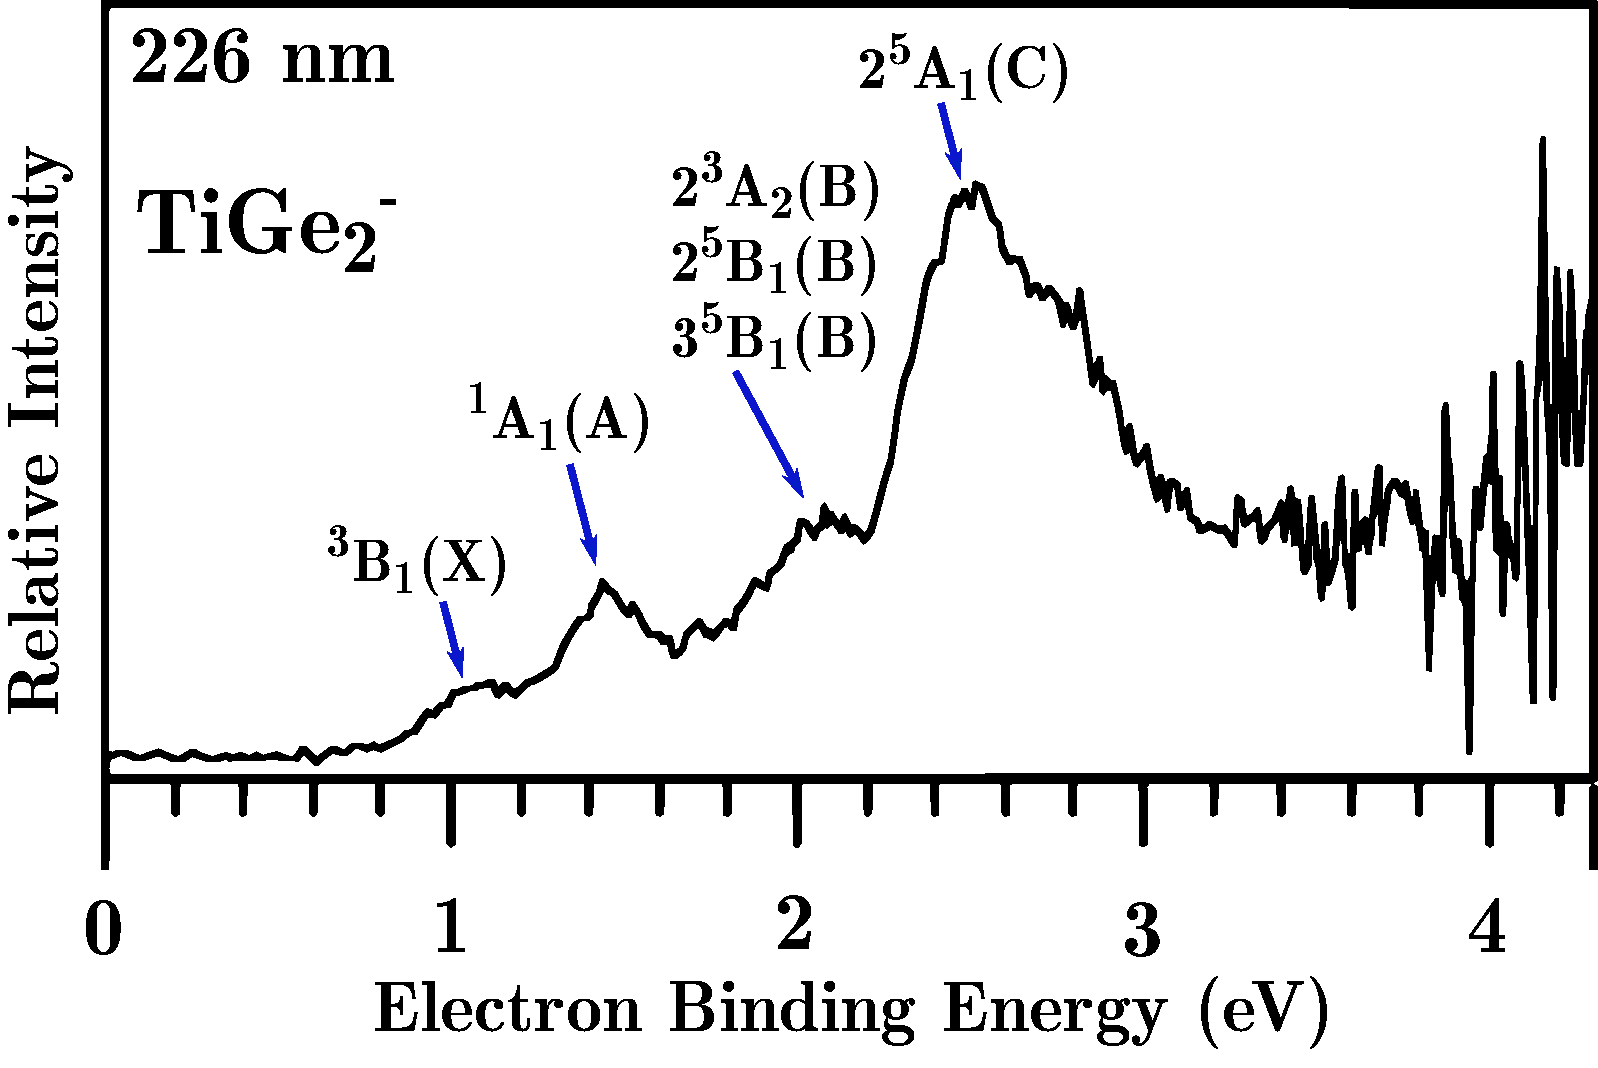
\includegraphics[width=0.5\textwidth]{Spectrum}
	\caption{Experimental anion \acrshort{pe} spectrum of \ch{TiGe2-} (reproduced with permission from ref \citenum{c4:22}, Copyright 2014, RSC Publisher).} 
	\label{fig4:spectrum}
\end{figure} 



\begin{table}[htb!]
	\centering
	\begin{threeparttable}
	\caption{Calculated \acrshort{vde} of \ch{TiGe2-}}
	\label{tbl4:DE}
	\begin{tabular}{@{}ccccccc@{}}
	\toprule
	\multirow{2}{*}{state} & \multicolumn{5}{c}{\acrshort{vde} (eV)\tnote{(b)}}                   & \multirow{2}{*}{state transition} \\ \cmidrule(l){2-6} 
				  & M06L   & \acrshort{rccsd}(T) & \acrshort{nevpt2} & \acrshort{caspt2} & exptl.     &                  \\ \midrule
	$^1$A$_1$     & 1.48   & 1.57     & 1.51   & 1.38   & 1.44 (A)   & $^2$A$_1$ $\longrightarrow$ $^1$A$_1$        \\
				  & 1.51   & 1.54     & 1.53   & 1.34   &            & $^2$A$_2$ $\longrightarrow$ $^1$A$_1$        \\
	$^3$A$_1$     & 2.42   & 2.23     & 2.22   & 2.13   &            &                  \\
	$^3$B$_1$     & 1.18   & 1.35     & 1.10   & 0.96   & 1.06  (X)  & $^4$B$_1$ $\longrightarrow$ $^3$B$_1$        \\
				  & (1.15) & (1.34)   & (1.07) & (0.90) & (0.78) (X) & $^4$B$_1$ $\longrightarrow$ $^3$B$_1$        \\
				  & 0.94   & 1.33     & 1.21   & 0.92   &            & $^2$A$_2$ $\longrightarrow$ $^3$B$_1$        \\
				  & (0.82) & (1.14)   & (1.01) & (0.82) &            & $^2$A$_2$ $\longrightarrow$ $^3$B$_1$        \\
	1$^3$B$_2$    & 1.35   & 1.37     & 1.18   & 0.98   &            &                  \\
	2$^3$B$_2$    &        &          &        & 0.92   & 1.06 (X)   & $^4$B$_1$ $\longrightarrow$ 2$^3$B$_2$       \\
	3$^3$B$_2$    &        &          &        & 1.69   &            &                  \\
	1$^3$A$_2$    & 1.95   & 2.00     & 2.11   & 1.99   &            &                  \\
	2$^3$A$_2$    &        &          &        & 1.90   & 2.05 (B)   & $^4$B$_1$ $\longrightarrow$ 2$^3$A$_2$       \\
	3$^3$A$_2$    &        &          &        & 1.48   &            &                  \\
	1$^5$A$_1$    & 2.23   & 2.47     & 2.22   & 2.03   &            &                  \\
	2$^5$A$_1$    &        & 2.62     &        & 2.31   & 2.49 (C)   & $^4$B$_1$ $\longrightarrow$ 2$^5$A$_1$       \\
	3$^5$A$_1$    &        &          &        & 2.94   &            &                  \\
	1$^5$B$_1$    & 2.60   & 2.78     & 2.56   & 2.42   &            &                  \\
	2$^5$B$_1$    &        &          &        & 2.03   & 2.05 (B)   & $^4$B$_1$ $\longrightarrow$ 2$^5$B$_1$       \\
	3$^5$B$_1$    &        &          &        & 2.16   & 2.05 (B)   & $^4$B$_1$ $\longrightarrow$ 3$^5$B$_1$       \\
	$^5$B$_2$     & 2.88   & 2.86     & 3.30   & 3.08   &            &                  \\
	$^5$A$_2$     & 3.13   & 3.04     & 3.58   & 3.16   &            &                  \\ \bottomrule
	\end{tabular}
	\begin{tablenotes}
		\item[(b)] Values without \acrshort{zpe} corrections, calculated at single-reference methods (M06-L, \acrshort{rccsd}(T)) and second-order perturbation theories (\acrshort{nevpt2} and \acrshort{caspt2}) on the basis of \acrshort{casscf} wave functions. \acrshort{caspt2}-optimized geometries of final states are used for all \acrshort{vde} calculations. All single-reference methods and \acrshort{nevpt2} employ the quintuple-$\zeta$ basis set aug-cc-pV5Z-DK. \acrshort{caspt2} energies are computed with the \acrshort{ano}-RCC basis set used in geometry optimizations. Values in parentheses are adiabatic \acrshort{ade}s calculated with the use of \acrshort{caspt2}-optimized geometries of involving states.
	\end{tablenotes}
	\end{threeparttable}
	\end{table}





In general, two types of one-electron detachments can be theoretically predicted, as noted in Table \ref{tbl4:ldconfig}. The ionization of one electron occurs, first from titanium's 4s and 3d orbitals, and second from germanium's 4p orbitals. Conventionally, the lowest ionization band X in an anion \acrshort{pe} spectrum is the result of one-electron transition between the anionic and neutral ground states. For the case of \ch{TiGe2-}, the X band can unambiguously be assigned to the electronic transition $^4$B$_1$ $\longrightarrow$ $^3$B$_1$, in which a 4s electron of titanium is detached under the laser beam of the photon. 




A closer look at the \acrshort{ade}s (Table \ref{tbl4:DE}, values in parentheses) reveals that all single-reference methods substantially overestimate \acrshort{ade}s in comparison to the experimental value. To be more detailed, the experimental \acrshort{ade} is 0.78 eV, while the M06-L and \acrshort{rccsd} values are 1.15 and 1.34 eV, respectively. On the other hand, the \acrshort{caspt2} estimate of 0.90 eV for this \acrshort{ade} is 0.12 eV larger than the experimental one. The \acrshort{nevpt2} \acrshort{ade} is larger than the \acrshort{caspt2} \acrshort{ade} by an amount of 0.17 eV. In comparison to experiment, the \acrshort{nevpt2} value is not in good agreement with experiment, even though its deviation is within the error bar. Clearly, neither \acrshort{dft} nor \acrshort{rccsd}(T) methods are able to reproduce the \acrshort{ade} of the X band on the basis of the electronic transition $^4$B$_1$ $\longrightarrow$ $^3$B$_1$. This result makes us carefully reconsider the experimental band X of the \acrshort{pe} spectrum.




The X band has not been well-resolved and is not clear enough to be a normal \acrshort{pe} band (Figure \ref{fig4:spectrum}). Thus, it would lead to a less precise determination of the \acrshort{ade} value. Although all of the states of \ch{TiGe2$^{-/0}$} bear multireference features, this is the lowest-lying band, and an assignment for this X band is rather straightforward without much doubt of the basis of two ground states. Turning to the computed \acrshort{vde}s for this band, multireference wave function methods \acrshort{nevpt2} and \acrshort{caspt2} again prove their capability in dealing with multireference systems like \ch{TiGe2$^{-/0}$}. Indeed, while \acrshort{nevpt2} reproduces a \acrshort{vde} of 1.10 eV, which is only 0.04 eV higher than the experimental \acrshort{vde} of 1.06 eV, \acrshort{caspt2} gives a deviation of 0.10 eV below the experimental \acrshort{vde}. Of the single-reference methods, the M06-L functional seems to be a good option for reproducing the X band \acrshort{vde} with a deviation of 0.12 eV. 





The situation becomes more interesting as another electronic transition $^4$B$_1$ $\longrightarrow$ 2$^3$B$_2$ starting from the anionic ground state involves a detachment energy of 0.92 eV at the \acrshort{caspt2} level, which lies in the region of the X band. However, the leading configuration of the final state 2$^3$B$_2$ has a coefficient weight of only 41\%. Therefore, this state does not strongly contribute to the photodetachment signal observed. If the $^2$A$_2$ state, another nearly degenerate state of the anionic state $^4$B$_1$ at both \acrshort{caspt2} and \acrshort{nevpt2} levels, is somehow populated in experiment, the transition $^2$A$_2$ $\longrightarrow$ $^3$B$_1$ should be observable in the spectrum. Because all of the \acrshort{ade}s and \acrshort{vde}s predicted by \acrshort{caspt2} and \acrshort{nevpt2} methods place signals of this transition in the X band's range, its intensity is expected to be in part overshadowed by signals from the transition $^4$B$_1$ $\longrightarrow$ $^3$B$_1$. Overall, three electronic transitions can contribute to the X band, in which the ground-ground transition $^4$B$_1$ $\longrightarrow$ $^3$B$_1$ is mainly responsible for the observed intensity.





Starting from the $^4$B$_1$, the next vertical \acrshort{ie} is estimated to be $\sim$2.0 eV (\acrshort{caspt2}). Indeed, seven final low-lying neutral states are positioned for this electron detachment (cf. Table \ref{tbl4:DE} for these neutral states). However, only three of them, 2$^3$A$_2$, 2$^5$B$_1$, and 3$^5$B$_1$, are allowed by the selection rule as analyzed above. At first, similar \acrshort{ie}s of these states are quite surprising because the ionization processes occurring from two different formal types of orbitals with different levels of energy, 3d (14b$_2$) orbitals of Ti for 2$^3$A$_2$ and 4p (17a$_1$ and 18a$_1$) orbitals of the ligand \ch{Ge2} for 2$^5$B$_1$ and 3$^5$B$_1$, need equal amounts of photon energy (2.0 eV). Nevertheless, a closer look at the pseudonatural orbitals can explain the situation. As a matter of fact, the ionized orbitals are not pure 3d or 4p orbitals. On the one hand, two ionized orbitals $\sigma_g$ (17a$_1$) and $\pi_{4p_z}$ (18a$_1$) have significant contributions from the 4s and 3d \acrshort{ao}s, and on the other hand, 3d$_{yz}$ (14b$_2$) is interfered substantially with the 4p$_z$ orbital of \ch{Ge2} (cf. Figure \ref{fig4:orbs} for more intuitive plots). Such contamination elevates energy levels of the \acrshort{mo}s $\sigma_g$ (17a$_1$) and $\pi_{4p_z}$ (18a$_1$) and reduces that of the 3d$_{yz}$ (14b$_2$) to new levels. As a consequence, three related ionization processes $^4$B$_1$ $\longrightarrow$ 2$^3$A$_2$, $^4$B$_1$ $\longrightarrow$ 2$^5$B$_1$, and $^4$B$_1$ $\longrightarrow$ 3$^5$B$_1$ are computed to have \acrshort{vde}s of 1.90, 2.03, and 2.16 eV, which all correspond to the experimental \acrshort{vde} of 2.05 eV of the B band. Because all three transitions start from the anionic ground state and are totally allowed by selection rules, they are likely to be simultaneously responsible for the experimental B band.







Beyond the B band, there is one band with higher detachment energy. This band has the highest experimental \acrshort{ie} of 2.49 eV. Because it has a high \acrshort{vde}, one-electron detachments underlying this band are expected to originate from the ligand orbitals. Correspondingly, our electronic analysis using the active space of \acrshort{casscf} calculations proves that a one-electronic transition can give a high \acrshort{ie} corresponding to the C band. This electronic transition, namely, $^4$B$_1$ $\longrightarrow$ 2$^5$A$_1$, is the result of one-electron removals from the $\pi_{4p_x}$ orbital of $^4$B$_1$. Unlike the features of other \acrshort{mo}s originating from the \ch{Ge2} moiety, the $\pi_{4p_x}$ orbital is purely from 4p$_x$. Thus, photodetachment of one electron from this \acrshort{mo} is predicted to need a larger energy than that from the $\sigma_g$ (17a$_1$) and $\pi_{4p_z}$ (18a$_1$). The \acrshort{caspt2} \acrshort{vde} of this transition (2.31 eV) is $\sim$0.18 eV smaller than the experimental value of 2.49 eV. The \acrshort{rccsd}(T) value of 2.62 eV is $\sim$0.13 eV above the experimental value, and this supports our attribution of the neutral state 2$^5$A$_1$ to the C band. In this context, the transition $^4$B$_1$ $\longrightarrow$ 2$^5$A$_1$ is a key contributor to the C band appearance.






There is still one unsolved band, which is the A band characterized by a \acrshort{vde} of 1.44 eV in the experimental \acrshort{pe} spectrum of \ch{TiGe2-}. All possible one-electron transitions starting from the state $^4$B$_1$ were already taken into account to assign other bands of the spectrum. In addition, no appropriate allowed transitions would correspond to this band energetically. Therefore, the degenerate state $^2$A$_1$ of the anionic ground state can now be invoked as the likely initial state from which one-electron ionization can occur. As the \acrshort{ie} associated with the A band is not so high (1.44 eV), one electron is expected to be removed from a 4s or a 3d orbital of titanium. This likely happens in the electronic transition $^2$A$_1$ $\longrightarrow$ $^1$A$_1$. More importantly, all predicted \acrshort{vde}s of this transition (in Table \ref{tbl4:DE}), at either single-reference or \acrshort{nevpt2} and \acrshort{caspt2} levels, are in good correlation with the experimental \acrshort{vde} of 1.44 eV. Deviation of theoretical estimates is around 0.10 eV. Accordingly, the A band is ascribed to the emergence of the low-spin state $^1$A$_1$. This result is quite similar to the situation of anionic vanadium dicarbide where a nearly degenerate anionic ground state is experimentally populated and gives rise to \acrshort{pe} bands. \cite{c4:44} Another electronic transition $^2$A$_2$ $\longrightarrow$ $^1$A$_1$ should also be mentioned because it is totally allowed by transition rules and has a predicted \acrshort{vde} properly corresponding to the A band. Nevertheless, this transition originating from the less populated state $^2$A$_2$ cannot substantially affect the intensity of the transition $^2$A$_1$ $\longrightarrow$ $^1$A$_1$.





\subsection{Franck-Condon Factor Simulations}


As seen previously, three of the four bands in the \acrshort{pe} spectrum of \ch{TiGe2-} are proved to be the results of more than one electronic transitions. The only band purely caused by a one-electron transition is the C band. Complicated contributions of multiple transitions to a band make multidimensional Franck-Condon factor simulations more difficult to give accurate reflection to a specific experimental band. Therefore, to simulate \acrshort{pe} bands of \ch{TiGe2-} more accurately, normal coordinates and vibrational frequencies of all accessible states underlying and/or contributing to these bands are utilized to calculate multidimensional Franck-Condon factors with up to 15 quanta. Technically, the vibrations of first two bands (X and A) are accessible, and hence, the simulations are conducted for these two bands. For the X band, two electronic transitions including $^4$B$_1$ $\longrightarrow$ $^3$B$_1$ and $^2$A$_2$ $\longrightarrow$ $^3$B$_1$ are simulated, and for band A, Franck-Condon factor integration of two one-electron detachments $^2$A$_1$ $\longrightarrow$ $^1$A$_1$ and $^2$A$_2$ $\longrightarrow$ $^1$A$_1$ is performed. In doing so, vibrational frequencies of all electronic states underlying bands X and A need to be observed, and these values obtained at the numerical \acrshort{caspt2} level are given in Table \ref{tbl4:feq}. Simulations of the Franck-Condon factor also need equilibrium geometries of involved states given in Table \ref{tbl4:RE}. Simulation results are illustrated in Figure \ref{fig4:FC}.






\begin{table}[htbp!]
	\centering
	\caption{Vibrational frequencies of involving states underlying two X and A bands in the \acrshort{pe} spectrum calculated at the \acrshort{caspt2} level of theory}
	\label{tbl4:feq}
	\begin{tabular}{@{}llll@{}}
	\toprule
	state & \acrshort{caspt2} frequency (cm$^{-1}$) & band & ionization \\ \midrule
	$^4$B$_1$   & 184, 277, 354           &      &            \\
	$^2$A$_1$   & 200, 238, 369           &      &            \\
	$^2$A$_2$   & 211, 271, 362           &      &            \\
	$^3$B$_1$   & 217, 226, 339           & X    & $^4$B$_1$ $\longrightarrow$ $^3$B$_1$  \\
		    &                             & X    & $^2$A$_2$ $\longrightarrow$ $^3$B$_1$  \\
	$^1$A$_1$   & 208, 242, 348           & A    & $^2$A$_1$ $\longrightarrow$ $^1$A$_1$  \\
		    &                             & A    & $^2$A$_2$ $\longrightarrow$ $^1$A$_1$  \\ \bottomrule
	\end{tabular}
	\end{table}






\begin{figure}[htb!]
	\centering
	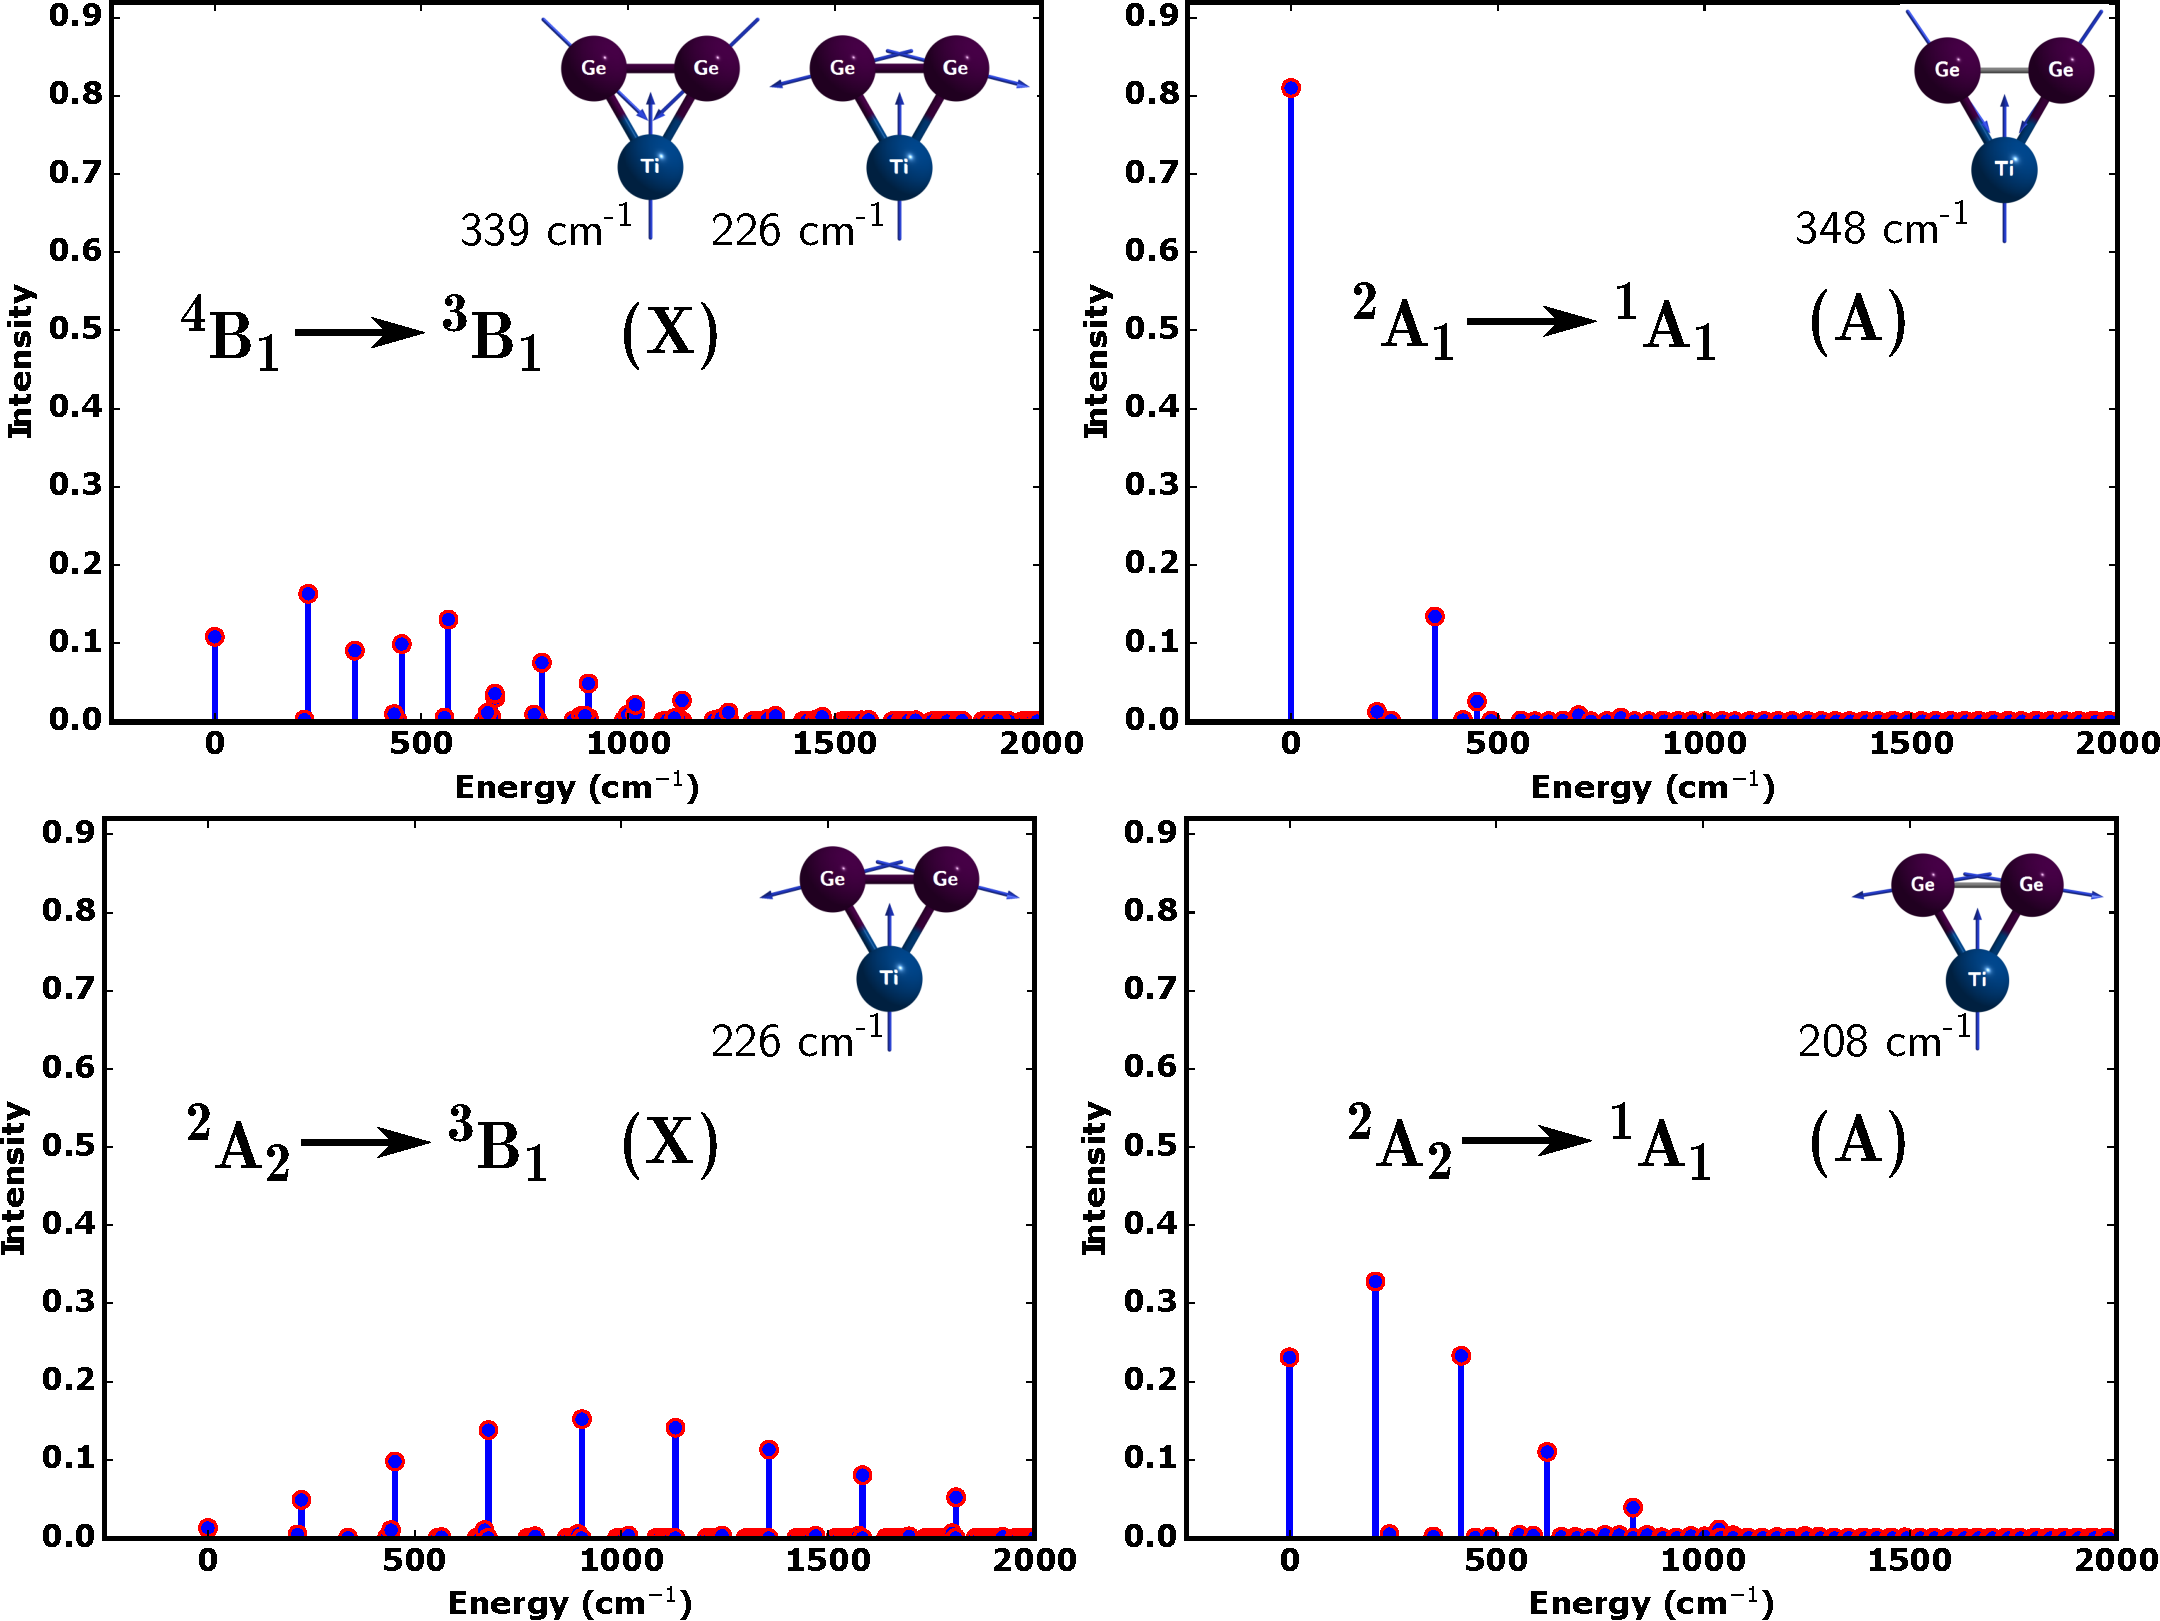
\includegraphics[width=\textwidth]{FC-simulation}
	\caption{Franck-Condon factor simulations of two bands X and A making use of \acrshort{caspt2} vibrational frequencies given in Table \ref{tbl4:feq} and of related equilibrium geometries in Table \ref{tbl4:RE}. Each band is simulated with two simultaneous electronic transitions.} 
	\label{fig4:FC}
\end{figure} 




Our Franck-Condon factor simulations are in excellent agreement with both experimental X and A bands in regard to relative intensities between both bands. Apparently, the intensities of two simulated progressions underlying the X band are quite low in comparison to those of the A band. This obvious relative intensity is experimentally observed in the \ch{TiGe2-} \acrshort{pe} spectrum displayed in Figure \ref{fig4:spectrum}. The X band is characterized with quite low intensity because of the considerable difference in equilibrium geometries (cf. Table \ref{tbl4:RE}) between the initial and final states underlying this band. Franck-Condon factor simulations also reveal more detailed information about the vibrational modes of final states participating in electronic transitions. In particular, all involved vibrational modes of final states include the vibration of titanium. This vibration is actually expected upon knowing about the types of electrons being removed from initial states. In all simulated progressions, one-electron detachments are determined to arise from 4s and 3d orbitals of titanium. Such ionizations of metallic electrons essentially provoke vibrations of titanium. Vibrational frequencies and associated normal modes chiefly making Franck-Condon factor integrals significant are given in the insets in Figure \ref{fig4:FC}.




\section{Concluding Remarks}



By employing a combination of different quantum chemical methods, the electronic structures of the triatomic species \ch{TiGe2^{-/0}} were thoroughly studied. Most states of \ch{TiGe2^{-/0}} appearing in the anion \acrshort{pe} experiment have multireference features. With the support from multireference wave functions, electronic structures of all states underlying the anion \acrshort{pe} spectrum were described. Our results firmly established that the ground state of the anion \ch{TiGe2-} is the high-spin state $^4$B$_1$. This conclusion disagrees with a previous theoretical study using \acrshort{dft} methods (B3LYP and HSE06 functionals), which concluded that $^2$A$_2$ is the anionic ground state.




Two other nearly degenerate anionic states $^2$A$_1$ and $^2$A$_2$ could be populated during the experiment, in which $^2$A$_1$ was proved to be the initial state for band A in the \acrshort{pe} spectrum of \ch{TiGe2-} while the other one is likely lesser populated but can affect the width of the observed bands.



Both the anion and neutral have several nearly degenerate states that significantly participate in the formation of \acrshort{pe} bands. Four bands in the spectrum of \ch{TiGe2-} were proved to originate from the two most likely degenerate states $^4$B$_1$ and $^2$A$_1$, and state $^2$A$_2$ could also affect the first two X and A bands. More specifically, the X, B, and C bands were mainly attributed to electronic transitions starting from the anionic ground state $^4$B$_1$, while the A band was ascribed to removal of one electron from the nearly degenerate state $^2$A$_1$ to form the neutral low-spin $^1$A$_1$.



Our Franck-Condon simulations of the first two X and A bands, on the basis of all possible transitions, gave additional understanding of normal modes and vibrational frequencies of the final neutral states. Concerning the quantum chemical methods, although multireference methods need to be used for this type of small clusters, our calculations suggested that the DFT/M06-L functional could be appropriate for treatment of systems such as \ch{TiGe2} if a single-reference method should be used.






%%%%%%%%%%%%%%%%%%%%%%%%%%%%%%%%%%%%%%%%%%%%%%%%%%
% Keep the following \cleardoublepage at the end of this file, 
% otherwise \includeonly includes empty pages.
%\cleardoublepage



\includebibliography
\printbibliography[heading=subbibliography] % print section bibliography

\end{refsection}